% !TeX root = ../main.tex
% Add the above to each chapter to make compiling the PDF easier in some editors.


\chapter{Introduction}\label{chapter:introduction}

Gesellschaft für Anlagen- und Reaktorsicherheit (GRS) conducts research and analysis in its fields of reactor safety, radioactive waste management,radiation and environmental protection. GRS is a leading expert organization in the field of radioactive waste management and nuclear safety.

The company consists of multiple management and scientific departments where each department is responsible for its specific fields. Working together the company has developed numerous different numerical applications and packages for the needs of nuclear safety analysis for the past 40 years. Bellow one can see the list of the  main scientific applications developed by GRS.
 
\begin{itemize}
	\item ASTEC: integral code for determination of the source term during core meltdown for the primary circuit and containment of LWRs
	\item ATHLET: thermohydraulic safety analyses for the primary circuit of  LWRs
	\item ATHLET-CD: analyses of accidents with core meltdown and fission product release for LWRs
	\item ATLAS: analysis simulator for interactive handling and visualisation of several computer codes
	\item COCOSYS: analyses of severe incidents in the containment of LWRs
	\item DORT/TORT: solution of time-dependant neutron transport equations for 2D/3D transients analyses
	\item QUABOX/CUBBOX: 3-D neutron kinetics core model
	\item SUSA: uncertainty and sensitivity analyses
	\item TESPA-ROD: core rod code for design basis accidents
\end{itemize}


Some applications can work together or with other external libraries and applications during a simulation with the aim of solving some multi-physical problems. Figure \ref{fig:applications} schematically shows an example of application coupling for an involved severe accident simulation.

As one can imagine each of those applications listed above needs a numerical solver to perform simulations. [solvers fast and parallel] Moreover, each scientific group has to keep developing and maintaining their own solvers which can be seen at the first glance as a work duplication. For that reason GRS made a decision to develop a so-called Numerical Toolkit (NuT) which had to become a universal collection of different and highly efficient numerical solvers. [That idea is not new and it has been use quite long time ago... something about PetSc]

\begin{figure}[htpb]
  \centering
  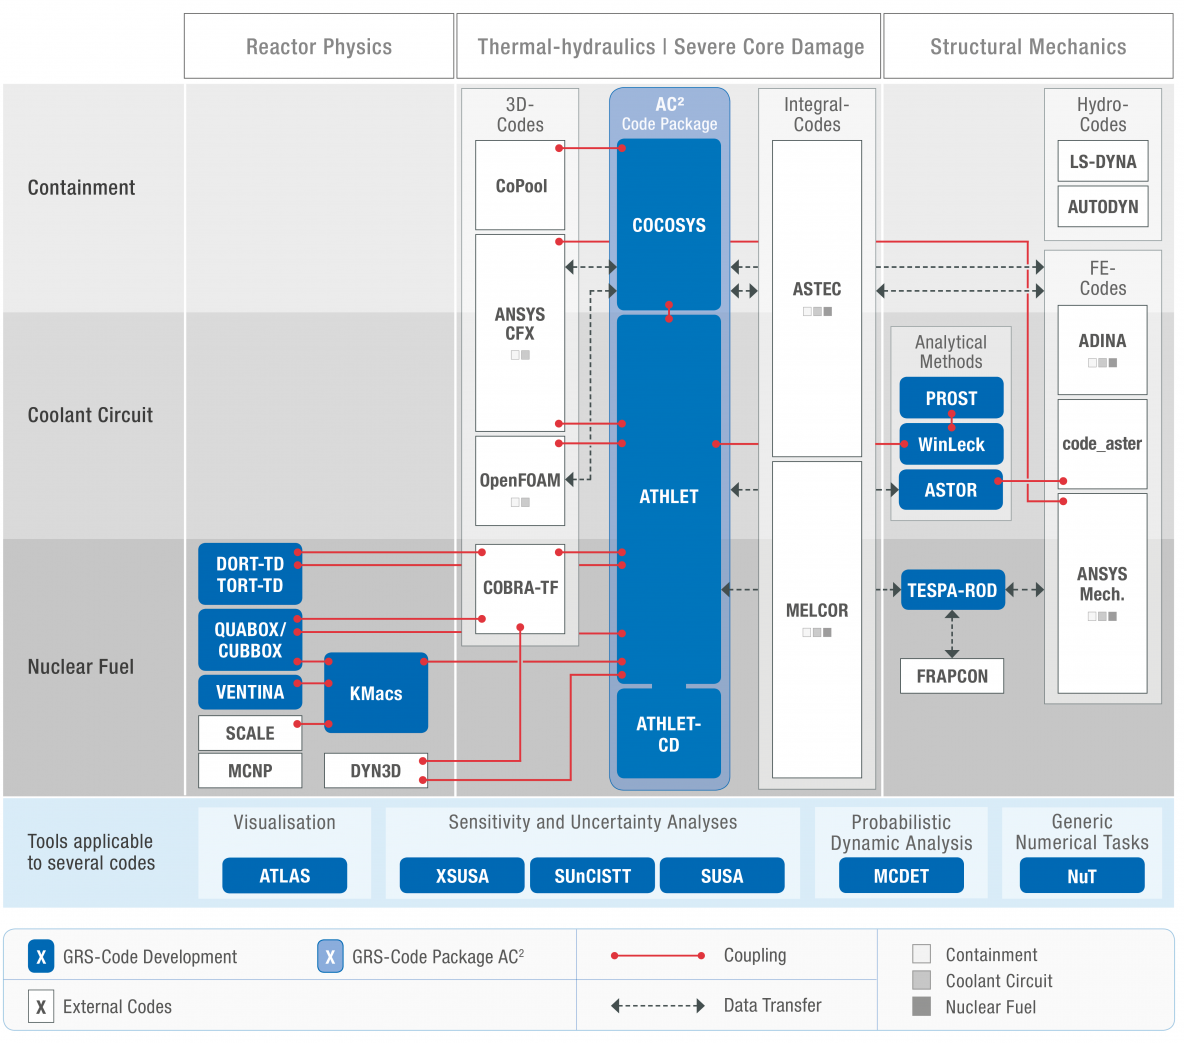
\includegraphics[width=0.8\textwidth]{figures/grs-application-coupling.png}
  \caption{An example of application coupling} \label{fig:applications}
\end{figure}